\documentclass{article}
\usepackage[textwidth=14cm]{geometry}
\usepackage[title]{appendix}
\usepackage[utf8]{inputenc}
\usepackage{amsmath}
\usepackage{physics}
\usepackage{graphicx}
\usepackage{mathtools}
\usepackage{subcaption}
\usepackage{hyperref}
\usepackage{fancyhdr}
\usepackage{float}
\usepackage{abstract}
\usepackage{lipsum}
\usepackage[english]{babel}
\usepackage[export]{adjustbox}[2011/08/13]
\usepackage{biblatex}
\addbibresource{Reference.bib}
\usepackage[flushleft]{threeparttable}
\usepackage{array,booktabs,makecell}
\usepackage{multirow}
\usepackage{floatrow}


\usepackage[table,xcdraw]{xcolor}
\renewcommand{\abstractname}{}
\renewcommand{\absnamepos}{empty} 
\hypersetup{
    colorlinks=true,
    linkcolor=blue,
    filecolor=magenta,      
    urlcolor=cyan,
}



\newcommand{\fsl}[1]{\ensuremath{\mathrlap{\!\not{\phantom{#1}}}#1}}% fsl{<symbol>}
\usepackage{tikz} 
\usetikzlibrary{shapes,arrows,positioning,automata,backgrounds,calc,er,patterns}
\usepackage{tikz-feynman,contour}
\tikzfeynmanset{compat=1.0.0}
\begin{document}
\title{FYS5555 Project 1}
\date{}
\begin{titlepage}
\centering
{\LARGE\bfseries FYS5555 Project 3}

\vspace{1cm}

{\Large Searching for two direct sleptons in a proton-proton collison using supervised machine learning}

\vspace{1.5cm}

{\large William Hirst}

\vspace{1cm}

{\bfseries Spring 2022}

\vspace{2cm}

\begin{figure}[H]
    \centering
    \includegraphics[width=0.8\linewidth]{Figures/Illustrations/signal.png}
    \label{fig:signal}
\end{figure}

\vfill

{\itshape University of Oslo}
\end{titlepage}
\newpage
\pagestyle{fancy}
\fancyfoot{}
\fancyfoot[R]{\thepage}

\begin{center}
\centering
\textit{
\lipsum[2]
}
\end{center}
\section{Introduction}
The standard model (SM) is perhaps one of the most successful scientific theories ever created. It accurately explains the interactions of leptons and quark as well as well as the force carrying particles which mediate said interactions. In 2012 the SM achieved one of its crowning achievements when discovering the Higgs boson. Much of the accolade was rightfully given to the theoretical work on the SM, but, another aspect of the discovery was equally importan. Data analysis was and is a crucial part of any new discovery in physics. One of the most important and exiting tools is machine learning.
\\
When on the search for beyond standard model (BSM)-physics, one often aims to search in regions where one suspects to find it. The traditional approach is to define regions by preforming rectangle cuts on event variables. In the case that the BSM is significantly different from the SM, this can be quite successfully. But, in the case that the two are relatively similar, rectangle cuts will not suffice. Machine learning aims to apply cuts that in practice are not (or at least do not seem) rectangle, but are curved. One often speaks about the machine learning creating a complex, curved region in the phase space spanned by the events.
\\
In this rapport I will use a mixed approach of rectangle cuts and machine learning and compare it to a strict rectangle cut approach in their ability to search for new physics. BSM-physics which will be the focus of this rapport will be Super Symmetry\footnote{More on the motivation behind super symmetry in section \ref{sec:SUSY}}. The methods compared in this raport will be tested on their ability to provide new information about the real data, either it be discovery or exclusion.
\\
In the theory section I will discuss the basis strategy of the search, Super symmetry and why it is worth the search, the different background-channels which will contribute to the analysis, the machine learning algorithm of choice and the statistical framework used in analysing the results. In the implementation section I will further explain the different methods used in the analysis, how I have chosen to handle the data as well as the steps involved in applying the machine learning framework. The results and discussion section will present all cuts used in defining different regions, the results from training the classifier, the results from applying each region, the final results from each search and will discuss possible ways forward. Finally all results and discussion, will be summarised in the conclusion section.
\section{Theory}
In this section I will discuss the necessary theory for both the physical analysis (supersymmetry, statistical tools ect.) as well as the tools need for the ML analysis. Note that the sections on ML methods is taken from my previous work in the articles \cite{FYSSTK} and \cite{HIGGS}.
\subsection{Basic search strategy}
In most attempts to search for BSM-physics the basic idea is to define a new model of interest and compare Monte Carlo data (MC) with with real data in designated regions we call signal regions (SR). To define these SR we use MC-data. As will be made clearer in later section, we want to define signal regions as a region in feature space with the most amount of predicted MC-data of the BSM physics of choice (signal) and the least amount of SM MC-data (background). Defining these regions can sometimes be done through classical rectangle cuts in certain features. Using machine learning in such searches allows us to define more sophisticated cuts based on trends in the features space that might be not visible to the human eye.
\subsection{Super symmetry}\label{sec:SUSY}
A supersymmetric theory has for many years been an interesting candidate for a new physics beyond the standard model. Supersymmetry (SUSY) aims to alter the standard model such that mass and force is treated equally. Supersymmetry suggests that each SM particle has an additional superpartner(SP) which we call a sparticle. The sparticles all differs with half a spin from the original SM particle. Because SUSY is a broken symmetry, sparticles are expected to be much higher than the corresponding SM masses, often in the range of 100-1000GeV. The difference in spin means that the SP of a fermion is a boson and the SP of a boson is a fermion. SUSY is a candidate to fix many problems in physics, some of which are; the hierarchy problem, fixing the mass of the higgs and possibly the mystery of dark matter.
\\
In this analysis I have chosen to search for supersymmetry through the signal of two direct sleptons decaying to a lepton and a neutralino. The process closely resembles the Drell-Yan production, but with additional neutralinos. The diagram is shown in figure \ref{fig:signal_f}. In the rapport only the sleptons $\tilde{e}$ and $\tilde{\mu}$ (SP of ${e}$ and ${\mu}$) will be considered.
\\
\begin{figure}[H]
    \centering
    \begin{tikzpicture}
    \begin{feynman}
        \vertex at (-1.75, 1.1) (i1) {\(P\)};
        \vertex at (-1.5, 1.) (i2);
        \vertex at (-1.525, 0.9) (i3) ;
        \vertex at (0.18, 1.1)  (a1);
        \vertex at (0.5, 1.) [blob] (a2) {\contour{white}};
        \vertex at (0.18, 0.9) (a3);
        
        \vertex at (-1.75, -1.1) (i4) {\(P\)};
        \vertex at (-1.5, -1.) (i5);
        \vertex at (-1.525, -0.9) (i6) ;
        \vertex at (0.18, -1.1)  (a4);
        \vertex at (0.5, -1.) [blob] (a5) {\contour{white}};
        \vertex at (0.18, -0.9) (a6);
        
        \vertex at (1.25, 0.0) (c);
        \vertex at (3., 0.0) (d);
        \vertex at (1,-0.5) (b);
        
        \vertex at (3.5, 1.) (f1) ;
        \vertex at (3.5,-1.) (f2);
        \vertex at (5.5, 1.5) (f3) {\(l^-\)};
        \vertex at (5.5, 0.5) (f4) {\(\tilde{\chi}_1^0\)};
        \vertex at (5.5, -0.5) (f5) {\(\tilde{\chi}_1^0\)};
        \vertex at (5.5, -1.5) (f6) {\(l^+\)};
        
    \diagram*{
        (i1) -- [lepton] (a1) ,
        (i2) -- [fermion] (a2) [blob],
        (i3) -- [lepton] (a3), 
        (a2) -- [fermion] (c) -- [boson] (d),
        (i4) -- [lepton] (a4) ,
        (i5) -- [fermion] (a5) [blob],
        (i6) -- [lepton] (a6), 
        (a5) -- [anti fermion] (c) -- [boson, edge label = {$Z,\gamma$}] (d),
        (d) -- [fermion, edge label =\(\tilde{l}^-\) ] (f1),
        (d) -- [fermion, edge label =\(\tilde{l}^+\) ] (f2),
        (f1) -- [fermion] (f3),
        (f1) -- [ghost] (f4),
        (f2) -- [anti fermion] (f6),
        (f2) -- [ghost] (f5),
        ;
    };
    \end{feynman}
    \end{tikzpicture}
    \caption{The Feynman diagram for the direct slepton signal channel.}
    \label{fig:signal_f}
\end{figure}
The different version of the direct slepton diagram are represented as different possibilities in the MC-data for the mass of the slepton and neutralinos. The masses of the slepton ranges from 100GeV to 700GeV and for the neutralinos the masses range from 1GeV to 300GeV.\\
Why search for neutralinos? Version of SUSY suggest an introduction of a new quantum number, R parity. The new quantum number suggests that the lightest neutralions do not decay into SM particles. Given it is neutral, this makes it a prime candidate for DM.

In this search
\subsection{Standard model background}
In the analysis of direct slepton signal there are several background channels of interest. In this rapport only a handful of the aforementioned channels were included in the rapport given the limits of computational power and time. The channels were included based on there relevance. 
\subsubsection{Dibson ($WW,WZ,ZZ$)}
Based on the results in the ATLAS paiper, \cite{Aad_2020} the diboson channels seems to be the largest source of background events. This is partly due to the variation of diagrams, but most importantly the resemblance to the signal diagram. Three diboson channels are included in the analysis; $WW$, $WZ$ and $ZZ$.
\\
In figure \ref{fig:WW} I have drawn the Feynman diagram of the WW channel. The figures shows two quark-annihilation forming a neutral boson, which decays into a pair of W-bosons. The W-boson later decay into a pair of charged and neutral leptons. 
\begin{figure}[H]
    \centering
    \begin{tikzpicture}
    \begin{feynman}
        \vertex at (-1.75, 1.1) (i1) {\(P\)};
        \vertex at (-1.5, 1.) (i2);
        \vertex at (-1.525, 0.9) (i3) ;
        \vertex at (0.18, 1.1)  (a1);
        \vertex at (0.5, 1.) [blob] (a2) {\contour{white}};
        \vertex at (0.18, 0.9) (a3);
        
        \vertex at (-1.75, -1.1) (i4) {\(P\)};
        \vertex at (-1.5, -1.) (i5);
        \vertex at (-1.525, -0.9) (i6) ;
        \vertex at (0.18, -1.1)  (a4);
        \vertex at (0.5, -1.) [blob] (a5) {\contour{white}};
        \vertex at (0.18, -0.9) (a6);
        
        \vertex at (1.25, 0.0) (c);
        \vertex at (3., 0.0) (d);
        \vertex at (1,-0.5) (b);
        
        \vertex at (3.5, 1.) (f1) ;
        \vertex at (3.5,-1.) (f2);
        \vertex at (5.5, 1.5) (f3) {\(l^-\)};
        \vertex at (5.5, 0.5) (f4) {\(\bar{\nu}\)};
        \vertex at (5.5, -0.5) (f5) {\(\nu\)};
        \vertex at (5.5, -1.5) (f6) {\(l^+\)};
        
    \diagram*{
        (i1) -- [lepton] (a1) ,
        (i2) -- [fermion] (a2) [blob],
        (i3) -- [lepton] (a3), 
        (a2) -- [fermion] (c) -- [boson] (d),
        (i4) -- [lepton] (a4) ,
        (i5) -- [fermion] (a5) [blob],
        (i6) -- [lepton] (a6), 
        (a5) -- [anti fermion] (c) -- [boson, edge label = {$Z,\gamma$}] (d),
        (d) -- [boson, edge label =\(W^-\) ] (f1),
        (d) -- [boson, edge label =\(W^+\) ] (f2),
        (f1) -- [fermion] (f3),
        (f1) -- [lepton] (f4),
        (f2) -- [anti fermion] (f6),
        (f2) -- [lepton] (f5),
        ;
    };
    \end{feynman}
    \end{tikzpicture}
    \caption{The Feynman diagram for the background diboson channel $WW$.}
    \label{fig:WW}
\end{figure}
In figure \ref{fig:WZ} I have drawn the Feynman diagram of WZ. The figure shows a up quark annihilating coupled to a W-boson and a down quark, and a anti-down quark coupled to a the aforementioned down quark and a Z-boson. The W-boson decays into a charged and neutral lepton pair and the Z can decay into a pair quarks or leptons. 
\begin{figure}[H]
    \centering
    \begin{tikzpicture}
    \begin{feynman}
        \vertex at (-1.75, 1.1) (i1) {\(P\)};
        \vertex at (-1.5, 1.) (i2);
        \vertex at (-1.525, 0.9) (i3) ;
        \vertex at (0.18, 1.1)  (a1);
        \vertex at (0.5, 1.) [blob] (a2) {\contour{white}};
        \vertex at (0.18, 0.9) (a3);
        
        \vertex at (-1.75, -1.1) (i4) {\(P\)};
        \vertex at (-1.5, -1.) (i5);
        \vertex at (-1.525, -0.9) (i6) ;
        \vertex at (0.18, -1.1)  (a4);
        \vertex at (0.5, -1.) [blob] (a5) {\contour{white}};
        \vertex at (0.18, -0.9) (a6);
        
        \vertex at (2.0, 1.) (c1);
        \vertex at (2.0, -1.) (c2);
        \vertex at (4.0, 1.) (d1);
        \vertex at (4.0, -1.) (d2);
        \vertex at (1,-0.5) (b);
        
        \vertex at (5.5, 1.5) (f3) {\(l^-\)};
        \vertex at (5.5, 0.5) (f4) {\(\bar{\nu}\)};
        \vertex at (5.5, -0.5) (f5) {\(l^-\)};
        \vertex at (5.5, -1.5) (f6) {\(l^+\)};
        
    \diagram*{
        (i1) -- [lepton] (a1) ,
        (i2) -- [fermion] (a2) [blob],
        (i3) -- [lepton] (a3), 
        (a2) -- [fermion, edge label = {$u$}] (c1) -- [boson, edge label = {$W^+$}] (d1),
        (i4) -- [lepton] (a4) ,
        (i5) -- [fermion] (a5) [blob],
        (i6) -- [lepton] (a6), 
        (c1) -- [fermion] (c2),
        (a5) -- [anti fermion,, edge label = {$\bar{d}$}] (c2) -- [boson, edge label = {$Z$}] (d2),
        (d1) -- [fermion] (f3),
        (d1) -- [lepton] (f4),
        (d2) -- [anti fermion] (f6),
        (d2) -- [fermion] (f5),
        ;
    };
    \end{feynman}
    \end{tikzpicture}
    \caption{Feynman diagram for the background diboson channel WZ.}
    \label{fig:WZ}
\end{figure}
In figure \ref{fig:ZZ} I have drawn the Feyman diagram of the ZZ-channel. The figure shows a diagram resembling that of the WZ-channel but with two Z-bosons. In this case the most relevant process for this analysis is the on where one of the Z-bosons decays into a pair of charged leptons and the other decays into a pair of neutral leptons. 
\begin{figure}[H]
    \centering
    \begin{tikzpicture}
    \begin{feynman}
        \vertex at (-1.75, 1.1) (i1) {\(P\)};
        \vertex at (-1.5, 1.) (i2);
        \vertex at (-1.525, 0.9) (i3) ;
        \vertex at (0.18, 1.1)  (a1);
        \vertex at (0.5, 1.) [blob] (a2) {\contour{white}};
        \vertex at (0.18, 0.9) (a3);
        
        \vertex at (-1.75, -1.1) (i4) {\(P\)};
        \vertex at (-1.5, -1.) (i5);
        \vertex at (-1.525, -0.9) (i6) ;
        \vertex at (0.18, -1.1)  (a4);
        \vertex at (0.5, -1.) [blob] (a5) {\contour{white}};
        \vertex at (0.18, -0.9) (a6);
        
        \vertex at (2.0, 1.) (c1);
        \vertex at (2.0, -1.) (c2);
        \vertex at (4.0, 1.) (d1);
        \vertex at (4.0, -1.) (d2);
        \vertex at (1,-0.5) (b);
        
        \vertex at (5.5, 1.5) (f3) {\(l^-\)};
        \vertex at (5.5, 0.5) (f4) {\(l^+\)};
        \vertex at (5.5, -0.5) (f5) {\(\nu\)};
        \vertex at (5.5, -1.5) (f6) {\(\bar{\nu}\)};
        
    \diagram*{
        (i1) -- [lepton] (a1) ,
        (i2) -- [fermion] (a2) [blob],
        (i3) -- [lepton] (a3), 
        (a2) -- [fermion, edge label = {$u$}] (c1) -- [boson, edge label = {$Z$}] (d1),
        (i4) -- [lepton] (a4) ,
        (i5) -- [fermion] (a5) [blob],
        (i6) -- [lepton] (a6), 
        (c1) -- [fermion] (c2),
        (a5) -- [anti fermion,, edge label = {$\bar{d}$}] (c2) -- [boson, edge label = {$Z$}] (d2),
        (d1) -- [fermion] (f3),
        (d1) -- [anti fermion] (f4),
        (d2) -- [lepton] (f6),
        (d2) -- [lepton] (f5),
        ;
    };
    \end{feynman}
    \end{tikzpicture}
    \caption{Feynman diagram for the background diboson channel ZZ.}
    \label{fig:ZZ}
\end{figure}

\subsubsection{$t\bar{t}$}
In figure \ref{fig:ttbar} I have drawn the Feynman diagram of the $t\bar{t}$-channel. Contrary to the diboson-channels, the proton-proton collision of the $t\bar{t}$-channel is initially mediated through gluons. The pair of gluons together form a $t\bar{t}$-pair. The $t\bar{t}$ decays into a jet-pair and two W-bosons. The W-bosons will each decay into a charged-neutral lepton-pair.

\begin{figure}[H]
    \centering
    \begin{tikzpicture}
    \begin{feynman}
        \vertex at (-1.75, 1.1) (i1) {\(P\)};
        \vertex at (-1.5, 1.) (i2);
        \vertex at (-1.525, 0.9) (i3) ;
        \vertex at (0.18, 1.1)  (a1);
        \vertex at (0.5, 1.) [blob] (a2) {\contour{white}};
        \vertex at (0.18, 0.9) (a3);
        
        \vertex at (-1.75, -1.1) (i4) {\(P\)};
        \vertex at (-1.5, -1.) (i5);
        \vertex at (-1.525, -0.9) (i6) ;
        \vertex at (0.18, -1.1)  (a4);
        \vertex at (0.5, -1.) [blob] (a5) {\contour{white}};
        \vertex at (0.18, -0.9) (a6);
        
        \vertex at (2.5, 1.0) (c1);
        \vertex at (2.5, -1.0) (c2);
        \vertex at (4., 1.) (d1);
        \vertex at (4., -1.) (d2);
        \vertex at (1,-0.5) (b);
        
        \vertex at (5.5, 1.5) (f3) {\(\bar{b}\)};
        \vertex at (5.5, 0.5) (f4) {\(\ W^-\)};
        \vertex at (5.5, -1.5) (f5) {\(b\)};
        \vertex at (5.5, -0.5) (f6) {\(W^+\)};

    \diagram*{
        (i1) -- [lepton] (a1) ,
        (i2) -- [fermion] (a2) [blob],
        (i3) -- [lepton] (a3), 
        (a2) -- [gluon] (c1) -- [anti fermion, edge label = {$\bar{t}$}] (d1),
        (i4) -- [lepton] (a4) ,
        (i5) -- [fermion] (a5) [blob],
        (i6) -- [lepton] (a6), 
        (c1) -- [fermion] (c2),
        (a5) -- [gluon] (c2) -- [fermion, edge label = {$t$}] (d2),
        (d1) -- [anti fermion] (f3),
        (d1) -- [boson] (f4),
        (d2) -- [fermion] (f5),
        (d2) -- [boson] (f6),
        ;
    };
    \end{feynman}
    \end{tikzpicture}
    \caption{The Feynman diagram for $t\bar{t}$-channel.}
    \label{fig:ttbar}
\end{figure}
\subsubsection{Single-top ($Wt$)}
In figure \ref{fig:singletop} I have drawn the Feynman diagram of the single-top-channel. The figure shows a bottom quark and a gluon that form a W-boson and a top-quark through another quark. The W-boson decays into a charged-neutral lepton pair and the top-quark will decay similarly to the top quarks discussed in the diagram for $t\bar{t}$.
\begin{figure}[H]
    \centering
    \begin{tikzpicture}
    \begin{feynman}
        \vertex at (-1.75, 1.1) (i1) {\(P\)};
        \vertex at (-1.5, 1.) (i2);
        \vertex at (-1.525, 0.9) (i3) ;
        \vertex at (0.18, 1.1)  (a1);
        \vertex at (0.5, 1.) [blob] (a2) {\contour{white}};
        \vertex at (0.18, 0.9) (a3);
        
        \vertex at (-1.75, -1.1) (i4) {\(P\)};
        \vertex at (-1.5, -1.) (i5);
        \vertex at (-1.525, -0.9) (i6) ;
        \vertex at (0.18, -1.1)  (a4);
        \vertex at (0.5, -1.) [blob] (a5) {\contour{white}};
        \vertex at (0.18, -0.9) (a6);
        
        \vertex at (2.0, 1.) (c1);
        \vertex at (2.0, -1.) (c2);
        \vertex at (4.0, 1.) (d1);
        \vertex at (4.0, -1.) (d2);
        \vertex at (1,-0.5) (b);
        
        \vertex at (5.5, 1.5) (f3) {\(l^-\)};
        \vertex at (5.5, 0.5) (f4) {\(\bar{\nu}\)};
        \vertex at (5.5, -1.5) (f5) {\(b\)};
        \vertex at (5.5, -0.5) (f6) {\(W^+\)};

        
    \diagram*{
        (i1) -- [lepton] (a1) ,
        (i2) -- [fermion] (a2) [blob],
        (i3) -- [lepton] (a3), 
        (a2) -- [fermion, edge label = {$b$}] (c1) -- [boson, edge label = {$W^-$}] (d1),
        (i4) -- [lepton] (a4) ,
        (i5) -- [fermion] (a5) [blob],
        (i6) -- [lepton] (a6), 
        (c1) -- [fermion] (c2),
        (a5) -- [gluon] (c2) -- [fermion, edge label = {$t$}] (d2),
        (d1) -- [fermion] (f3),
        (d1) -- [lepton] (f4),
        (d2) -- [fermion] (f5),
        (d2) -- [boson] (f6),
        
        ;
    };
    \end{feynman}
    \end{tikzpicture}
    \caption{The Feynman diagram for singletop-channel.}
    \label{fig:singletop}
\end{figure}
\subsubsection{W/Z+Jets}\label{subsec:WZjets}
In figure \ref{fig:WZ_jets} I have drawn one example of Feynman diagrams fro both the W- and Z+jets channel. The diagram shows two fermions that create a gluon and a Z- or W-boson through the t-channel. The gluon decays into a jet and the W- or Z-boson decays into a pair of leptons, either one or two charged. As is evident from the work made by ATLAS in articles like their work in 2020 \cite{Aad_2020}, normally in searches for direct sleptons, these channels can be easily cut. But, as will be discussed in later sections, the lack of certain features in the data will make the channels contribute an abnormal amount.
\begin{figure}[H]
    \centering
    \begin{tikzpicture}
    \begin{feynman}
        \vertex at (-1.75, 1.1) (i1) {\(P\)};
        \vertex at (-1.5, 1.) (i2);
        \vertex at (-1.525, 0.9) (i3) ;
        \vertex at (0.18, 1.1)  (a1);
        \vertex at (0.5, 1.) [blob] (a2) {\contour{white}};
        \vertex at (0.18, 0.9) (a3);
        
        \vertex at (-1.75, -1.1) (i4) {\(P\)};
        \vertex at (-1.5, -1.) (i5);
        \vertex at (-1.525, -0.9) (i6) ;
        \vertex at (0.18, -1.1)  (a4);
        \vertex at (0.5, -1.) [blob] (a5) {\contour{white}};
        \vertex at (0.18, -0.9) (a6);
        
        \vertex at (2.0, 1.) (c1);
        \vertex at (2.0, -1.) (c2);
        \vertex at (4.0, 1.) (d1);
        \vertex at (4.0, -1.) (d2);
        \vertex at (1,-0.5) (b);
        
        \vertex at (5.5, 1.5) (f3) {\(l^-\)};
        \vertex at (5.5, 0.5) (f4) {\(l^+/\bar{\nu}\)};
        \vertex at (5.5, -0.5) (f5) {\(b\)};
        \vertex at (5.5, -1.5) (f6) {\(\bar{b}\)};
        
    \diagram*{
        (i1) -- [lepton] (a1) ,
        (i2) -- [fermion] (a2) [blob],
        (i3) -- [lepton] (a3), 
        (a2) -- [fermion] (c1) -- [boson, edge label = {$Z/W^-$}] (d1),
        (i4) -- [lepton] (a4) ,
        (i5) -- [fermion] (a5) [blob],
        (i6) -- [lepton] (a6), 
        (c1) -- [fermion] (c2),
        (a5) -- [anti fermion] (c2) -- [gluon, edge label = {$G$}] (d2),
        (d1) -- [fermion] (f3),
        (d1) -- [anti fermion] (f4),
        (d2) -- [anti fermion] (f6),
        (d2) -- [fermion] (f5),
        ;
    };
    \end{feynman}
    \end{tikzpicture}
    \caption{Feynman diagram for the background channels W+jets and Z+jets.}
    \label{fig:WZ_jets}
\end{figure}
\subsection{Gradient-boosted trees \cite{HIGGS}}
Gradient-boosting is a machine learning algorithm which uses a collective of "weak" classifiers in order to create one strong classifier. In the case of gradient-boosted trees the weak classifiers are a collective of shallow trees, which combine to form a classifiers that allows for deeper learning. As is the case for most gradient-boosting techniques, the collecting of weak classifiers is an iterative process.
\\
We define an imperfect model $\mathcal{F}_m$, which is a collective of m number of weak classifiers, estimators. A prediction for the model on a given data-points, $x_i$ is defined as $\mathcal{F}_m(x_i)$, and the observed value for the aforementioned data is defined as $y_i$. The goal of the iterative process is to minimize some cost-function $\mathcal{C}$ by introducing a new estimator $h_m$ to compensate for any error, $\mathcal{C}(\mathcal{F}_m(x_i), y_i)$. In other words we define the new estimator as:
\begin{align}
    \tilde{\mathcal{C}}(\mathcal{F}_m(x_i), y_i) = h_m(x_i),
\end{align}
where we define $\tilde{\mathcal{C}}$ as some relation defined between the observed and predicted values such that when added to the initial prediction we minimize $\mathcal{C}$.
\\
Using our new estimator $h_m$, we can now define a new model as
\begin{align}
    \mathcal{F}_{m+1}(x_i) = \mathcal{F}_m + h_m (x_i).
\end{align}
The XGBoost \cite{XGB} framework used in this analysis enables a gradient-boosted algorithm, and was initially created for the Higgs ML challenge. Since the challenge, XGBoost has become a favorite for many in the ML community and has later won many other ML challenges. XGBoost often outperforms ordinary decision trees, but what is gains in results it looses in interpretability. A single tree can easily be analysed and dissected, but when the number of trees increases this becomes harder. 
\subsection{Discovery and exclusion}
As mentioned in previous sections, the main idea of the search is to define a region where we will compare the MC-background to the data and analyse any differences. Any analysis in the signal region hopes to either discovery or exclude certain BSM physics. The usual way of doing so is through statistics. In this rapport the statistical analysis will not be the focus and will therefore not be explained in heavy detail. Nonetheless there are certain expressions and terms that must still be defined.
\\
In the sake of a discovery one would hope to see an excess in the data, measure its significance and find the model best fitting to the excess. A significance of a discovery is measured by the relation between the background and the apparent signal. Given a signal region with $n_{obs}$ events of real data and b events of MC background, we can define the signal as $s = n_{obs}-b$. Then a significance of any signal, $Z$ is defined as 
\begin{align}
    Z = \frac{n_{obs}-b}{\sqrt{b}},
\end{align}
or 
\begin{align}
    Z = \frac{s}{\sqrt{b}}.
\end{align}
Introducing the possibility of uncertainty in the amount of background, $\delta b$ we can further define
\begin{align}\label{eq:Z}
    Z = \frac{s}{\sqrt{b+(\delta b)^2}}.
\end{align}
In physics one often deems the results a discovery if $Z$ is larger than 5.  Given a significance with no indication of discovery, we move over to the intent of exclusion.\\
In exclusion we are interested in studying the probability of a model which predicts a number of signal events s, given $n_{obs}$ real data events. To do so we will use Bayesian statistics.
\\
The probability of model predicting $s$ signal events in the signal region, given $n_{obs}$ event of real data is in bayesian statistics written as
\begin{align}\label{eq:bays}
    P(s|n_{obs}) = \frac{P(n_{obs}|s)P(s)}{P(n_{obs})}
\end{align}
Approximating the probability distribution with a Poisson distribution we can define this probability as
\begin{align}\label{eq:Pns}
    P(n_{obs}|s) = L(n_{obs},s)= (s+b)^{n_{obs}} \frac{e^{-(s+b)}}{n_{obs}!},
\end{align}
where b is the predicted background. 
\\
From this point we can define $s_{up}$ as being the upper limit of any signal, where any model that predicts $s>s_{up}$ is excluded. We define $s_{up}$ as
\begin{align}
    \int_0^{s_{up}} P(s|n_{obs})  = 0.95,
\end{align}
meaning that any $s>s_{up}$ is excluded within a $95\%$ confidence. If we assume flat prior both $P(n_{obs})$ and $P(s)$ are independent of s, and will act as normalization constants. Therefore we can calculate $s_{up}$ using equation \ref{eq:bays}. 
\\
To further extend this approach for HEP purposes we make the probability dependant of 4 parameters, the signal cross section $\sigma$, the background cross section $\sigma_{bkg}$,  the integrated luminosity $L_{int}$ (which for the sake of this rapport is $10fb^{-1}$) and the efficiency $\epsilon$. The efficiency in this case is equal to the fraction of signal before and after the different region requirements were applied. 
\\
We can define 
\begin{align}\label{eq:sb}
    s+b = L_{int} (\epsilon \sigma + \sigma_{bkg}).
\end{align}
Using equation \ref{eq:bays}, \ref{eq:Pns}, \ref{eq:sb} and marginalizing we can find a new expression for our original probability as
\begin{align}
    P(\sigma | n_{obs}) =N \int L\left(\sigma, L_{\text {int }}, \varepsilon, \sigma_{\mathrm{bkg}}\right) p\left(L_{\mathrm{int}}\right) p\left(\varepsilon\right) p\left(\sigma_{\mathrm{bkg}}\right) d L_{\mathrm{int}} d \varepsilon_{\mathrm{sig}} d \sigma_{\mathrm{bkg}},
\end{align}
where N is a normalization constant and the probability is now depndant on the signal cross section. To calculate expressions as the ones above and to find $s_{up}$ Monte carlo integration must be used. In this rapport I used the statistical framework created by Magnar Kopangen Bugge in the statisticsNotebook to calculate all limits.
\section{Implementation}
The cuts in the analysis are all chosen by me, although some are inspired by the work of Eirik Gramstad in his thesis from 2013 \cite{Gramstad:2013loc}.
\subsection{Cuts and signal regions}
In this rapport I will define 2 signal regions. Both signal regions will have a common base, which I will call the analysis region (AR). The AR will be defined making relatively loose cuts on the variables of the MC-data. This region will aim to remove unnecessary background processes and at the same time keep as much of the signal as possible, around $20-60\%$. The hope of these cuts is to leave only signal and irreducible background events left.
\\
The first signal region (SR2), will use AR as a base and add an additional cut from the ML output.  This region will be used in the statistical analysis for any results produced from our ML-model. The second signal region (SR2) will also use SR1 as a base, but will add additional cuts on the variables. These cuts will be much stricter to remove as much irreducible background as possible, and will as a consequence remove a larger amount of signal than both SR1 and SR2. 
\\
The purpose of SR1 and SR2 is to compare any result of detection or exclusion of BSM between a rectangle cut only approach to the machine learning approach. 
\subsection{Data handling}\label{sec:DH}
For training and testing of the XGBoost classifier I created three data sets; one training, one validation and one test. All the data sets are based on the AR (\ref{table:AR}). The training set consisted of $80\%$ of the data, saving the remaining $20\%$ for validation. Given the large amount of background, the data (both training and validation) was scaled such that the sum of the weights were equal for signal and background. This was done to ensure a realistic representation of the background data as well as making sure that the classifier is given a sufficient amount of signal. The final data-set (testing) consisted of all the background data and is used to visualize the the classifiers ability to act on all the SM MC-data.
\\
Additional to the imbalanced data-set, there was a problem with the weights produced by the MC-simulations, some of the weights were negative. The negative weight problem is a well known problem in the world of ML-analysis for HEP, and arise as a consequence of higher perturbative accuracy. For the purpose of visualising distributions, negative weights are not a problem. But, when using the weights in the training of the classifier, the XGBoost framework will not work. 
\\
How one chooses to deal with this problem can heavily effect results and many solution are suggested as a consequence. Given the time limitations of this rapport, the simplest solution was chosen. Namely, I chose to normalize all the weights as a whole, conserving the total sum of the weights and at the same time changing all negative signs. The simple procedure is shown bellow in equation \ref{eq:negw},
\begin{align}\label{eq:negw}
    w_i & = P \mid w_i \mid\,  \\
    P  & =  \sum_{j=0}^{N-1}\frac{ w_j}{\mid w_j \mid},
\end{align}
where $w_i$ is the weight of an event i, $i \in [0,N-1]$ and N equals the total number of events.
\subsection{The XGBoost-classifier}
For the case of this rapport, no gridsearch was used in finding hyper-parameters for the XGBoost-classifier. This was a conscience decision based on two reason. Firstly the data set used in this analysis is very large. Any gridsearch that would have any hope of finding optimal parameters would be very time consuming. Secondly the algorithm behind boosting, and especially in the XGBoost framework often means that the parameters in the classifier are not as crucial as in other methods such as deep networks. It is an unproven phenomenon that the XGBoost-classifier often prefers its default settings (see \cite{XGB} for full description). Therefore most of these parameters were used in the rapport with a couple exceptions.
\\
Some of the parameters were changed to either make the classifier faster, or based on previous experience i similar analysis. Firstly the learning rate was changed to $0.1$. Secondly the the $max\_depth$ of the classifier was changed to 3. Finally the weights of the classifier was set to the sum of the weights of signal divided by the sum of the weights of background. This was done as a suggestion by the XGBoost-contributors. Given the scaling of the weights this factor will be 1. 
\section{Results and discussion}
\subsection{Monte Carlo and Data}\label{subsec:MCandData}
Given the main ideas of the search is to compare MC to real data, one must first make sure that the MC-data in-fact resembles the real data. To do so I have plotted the distribution of 9 variables. In addition I plot the ratio of real data divided by MC for each bin. For practical purposes the contribution of SUSY signal is included in the distribution plot, but given the small amount of signal it will not effect the comparison. However the SUSY signal is not included in the ratio plot.
\\
In figure \ref{fig:var1} I have plotted the transverse momentum for the first \ref{fig:Cuts_pt1} and second lepton \ref{fig:Cuts_pt2}, missing transverse energy \ref{fig:Cuts_met}, dilepton mass \ref{fig:Cuts_mll} and the stransverse momentum \ref{fig:Cuts_T2}. In all the aforementioned figures we observe a clear similarity between the MC and real data. This is especially evident by studying the ratio-plots under each plot. Most of the ratios are located around, more so even for the bins with the highest number of events. From the ratio plots we also observe that the largest difference between MC and data happens for events with larger energy's/momentum.  
\\
\begin{figure}
    \makebox[\linewidth][c]{%
     \centering
     \begin{subfigure}[b]{.6\textwidth}
         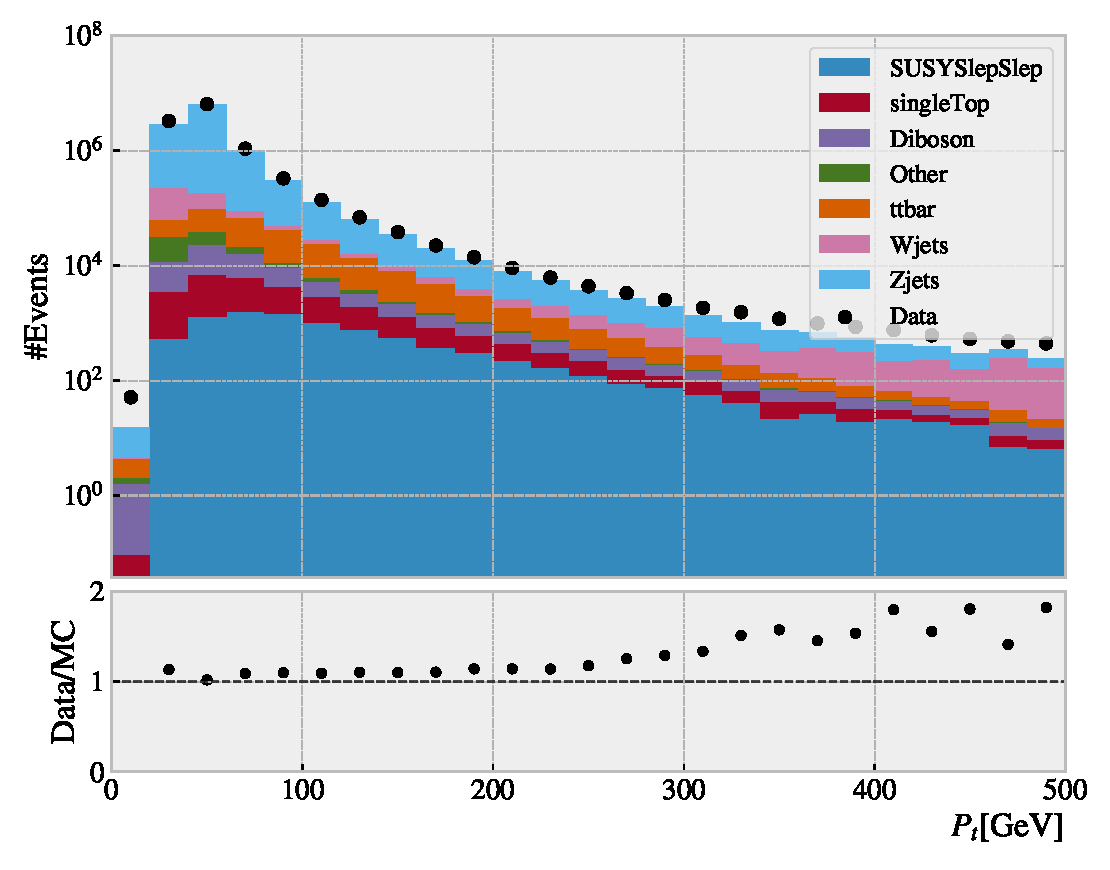
\includegraphics[width=\textwidth]{Figures/Cuts/p_t1.pdf} 
         \caption{}
         \label{fig:Cuts_pt1}
     \end{subfigure}
     \centering
     \begin{subfigure}[b]{.6\textwidth}
         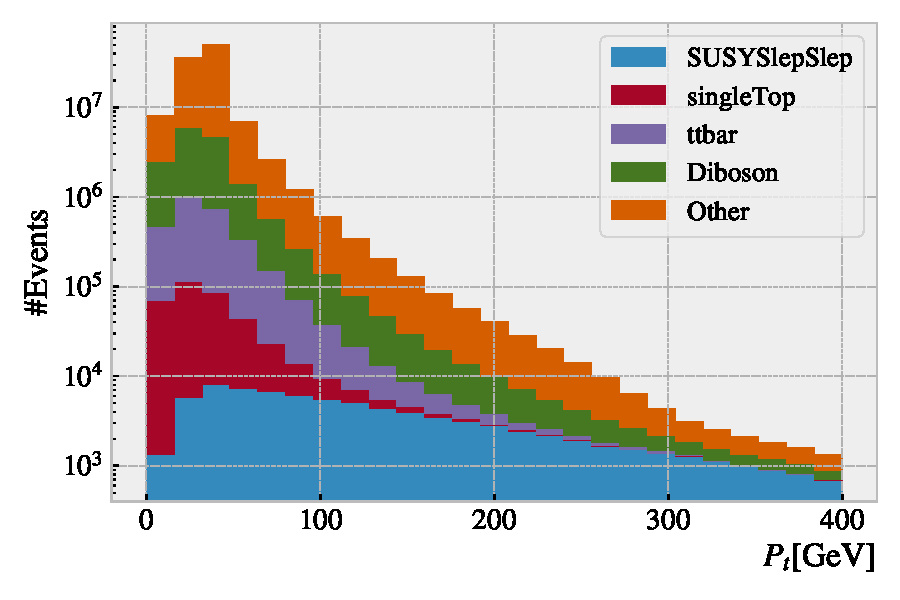
\includegraphics[width=\textwidth]{Figures/Cuts/p_t2.pdf} 
         \caption{}
         \label{fig:Cuts_pt2}
     \end{subfigure}
    }
     \makebox[\linewidth][c]{%
     \centering
     \begin{subfigure}[b]{.6\textwidth}
         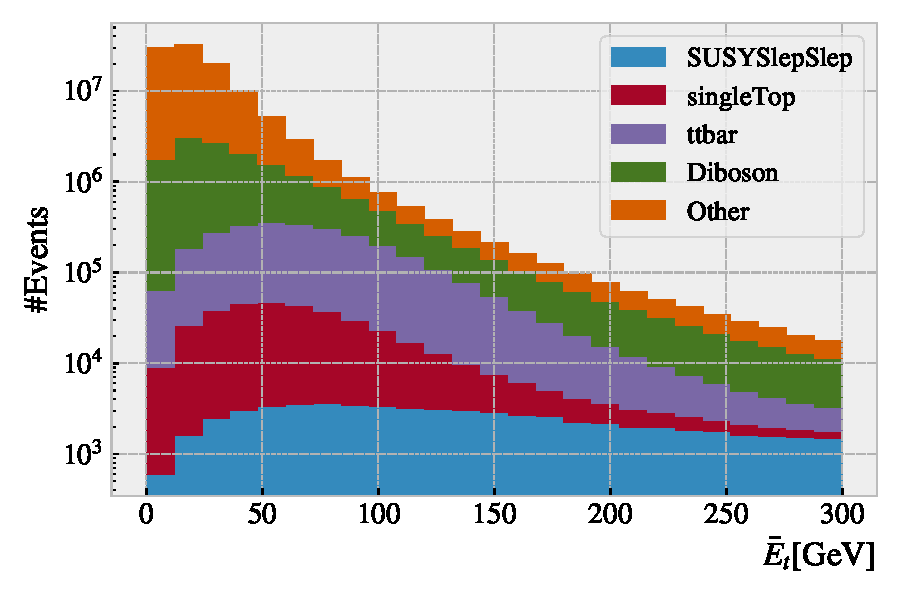
\includegraphics[width=\textwidth]{Figures/Cuts/MET.pdf} 
         \caption{}
         \label{fig:Cuts_met}
     \end{subfigure}
     \centering
     \begin{subfigure}[b]{.6\textwidth}
         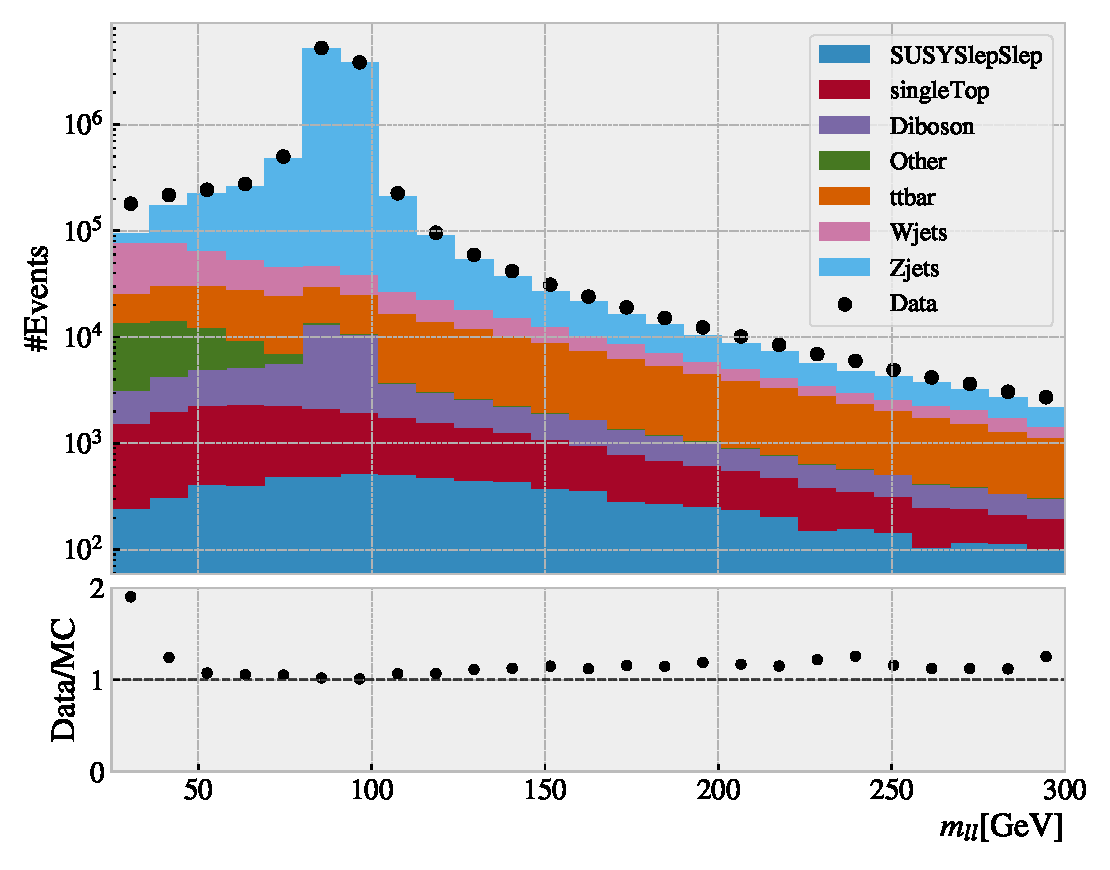
\includegraphics[width=\textwidth]{Figures/Cuts/mll.pdf} 
         \caption{}
         \label{fig:Cuts_mll}
     \end{subfigure}
    }
    \centering
    \makebox[\linewidth][c]{%
    \begin{subfigure}[b]{.6\textwidth}
         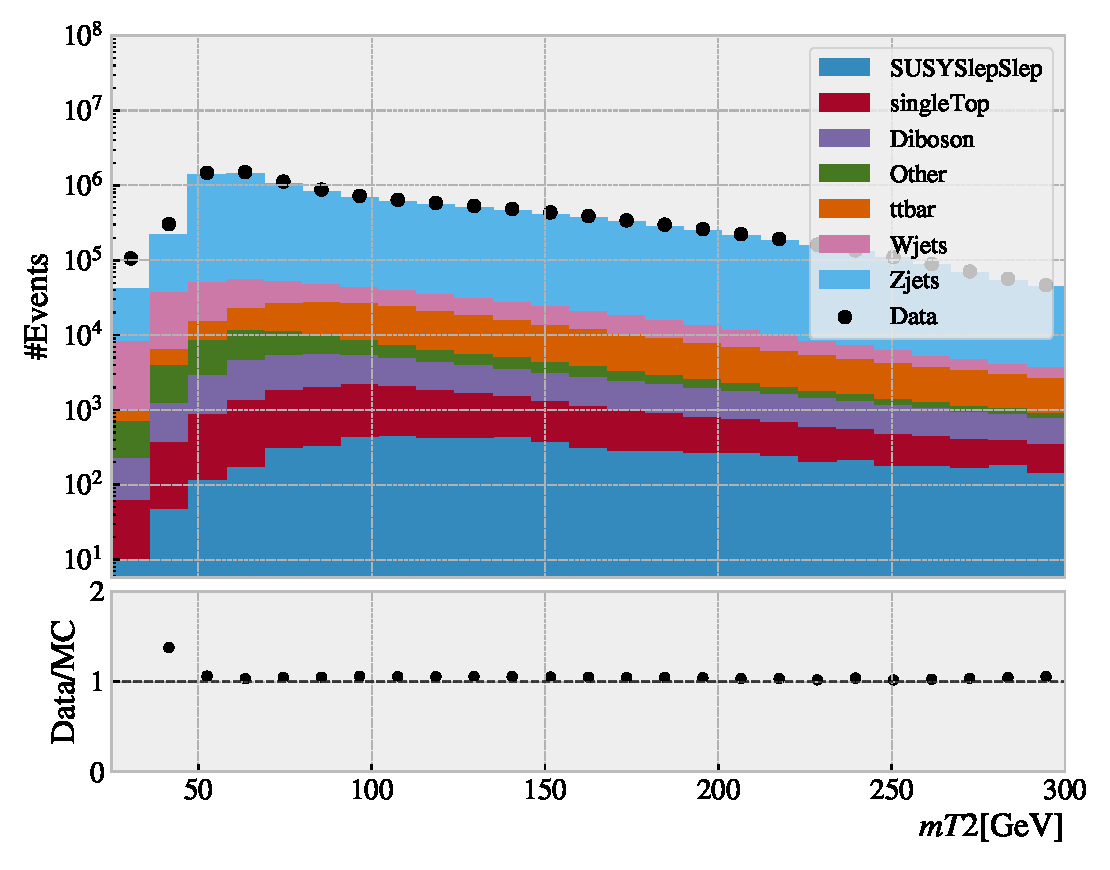
\includegraphics[width=\textwidth]{Figures/Cuts/mT2.pdf}
         \caption{}
         \label{fig:Cuts_T2}
    \end{subfigure}
    \begin{subfigure}[t]{0.6\textwidth}
                \vspace{-180 pt} 
                \captionsetup{width=.9\linewidth}
                \caption*{Figure 8: The distribution of transverse momentum of first \ref{fig:Cuts_pt1} and second \ref{fig:Cuts_pt2} lepton, missing transverse energy \ref{fig:Cuts_met}, dilepton mass \ref{fig:Cuts_mll} and the stransverse mass \ref{fig:Cuts_T2} for the MC and real data. Additionally the ratio of data over MC is plotted under each distribution histogram.
                }
    \end{subfigure}
     }
     \captionsetup{labelformat=empty}
    \caption{}
    \label{fig:var1}
\end{figure}

\begin{figure}
    \makebox[\linewidth][c]{%
     \centering
     \begin{subfigure}[b]{.6\textwidth}
         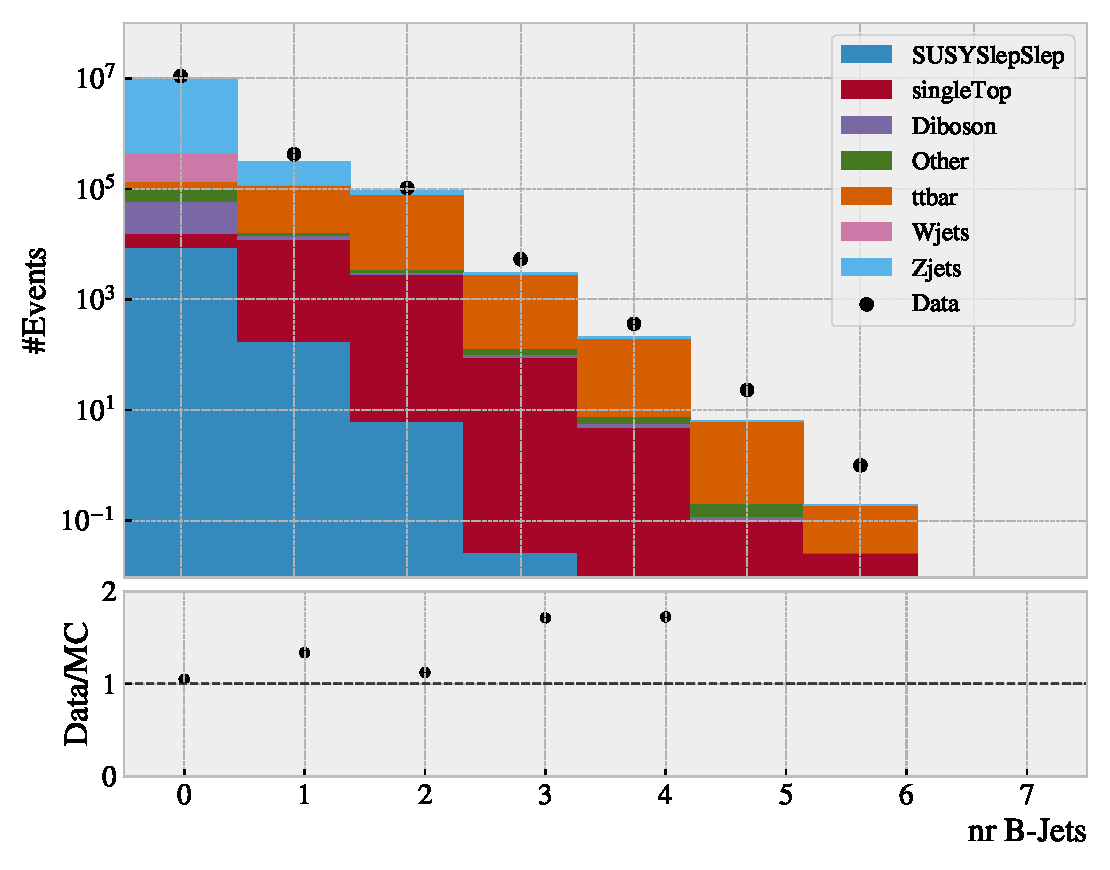
\includegraphics[width=\textwidth]{Figures/Cuts/bTag.pdf} 
         \caption{}
         \label{fig:Cuts_bTag}
     \end{subfigure}
     \centering
     \begin{subfigure}[b]{.6\textwidth}
         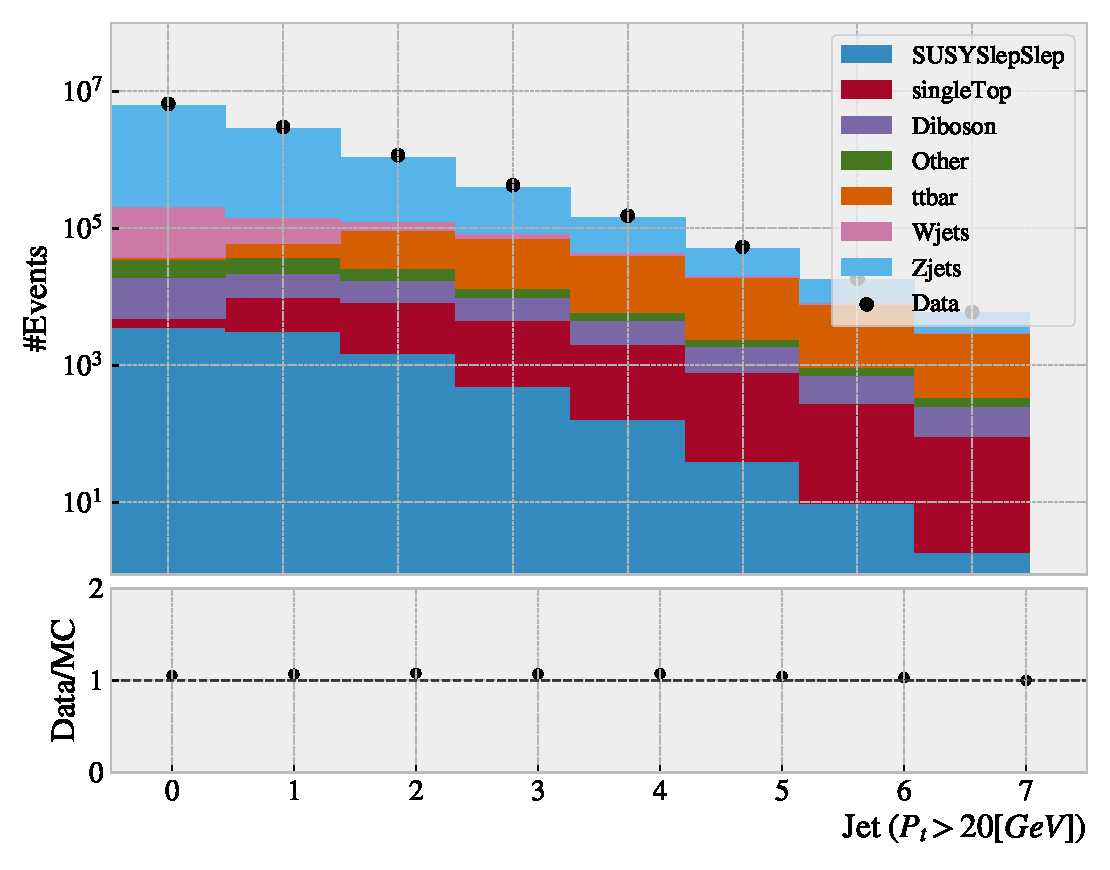
\includegraphics[width=\textwidth]{Figures/Cuts/njet20.pdf} 
         \caption{}
         \label{fig:Cuts_jet20}
     \end{subfigure}
    }
     \makebox[\linewidth][c]{%
     \centering
     \begin{subfigure}[b]{.6\textwidth}
         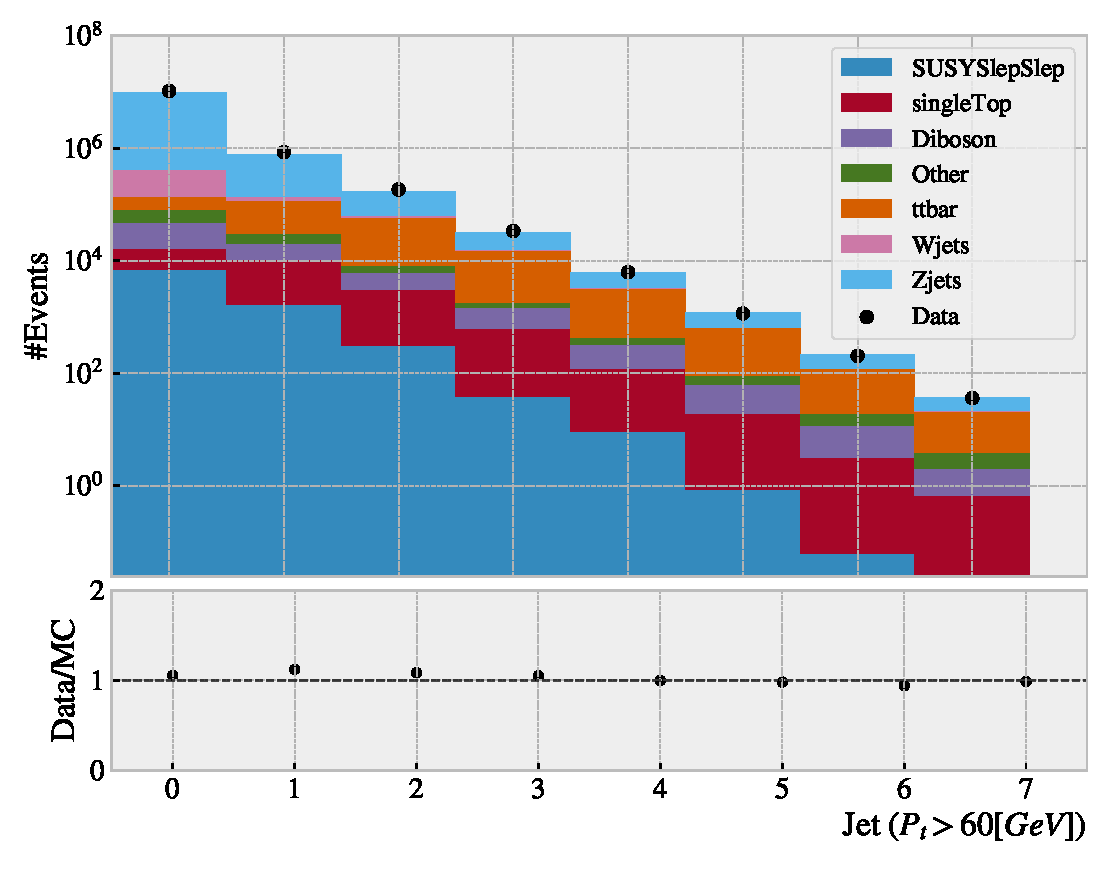
\includegraphics[width=\textwidth]{Figures/Cuts/njet60.pdf} 
         \caption{}
         \label{fig:Cuts_jet60}
     \end{subfigure}
     \centering
     \begin{subfigure}[b]{.6\textwidth}
         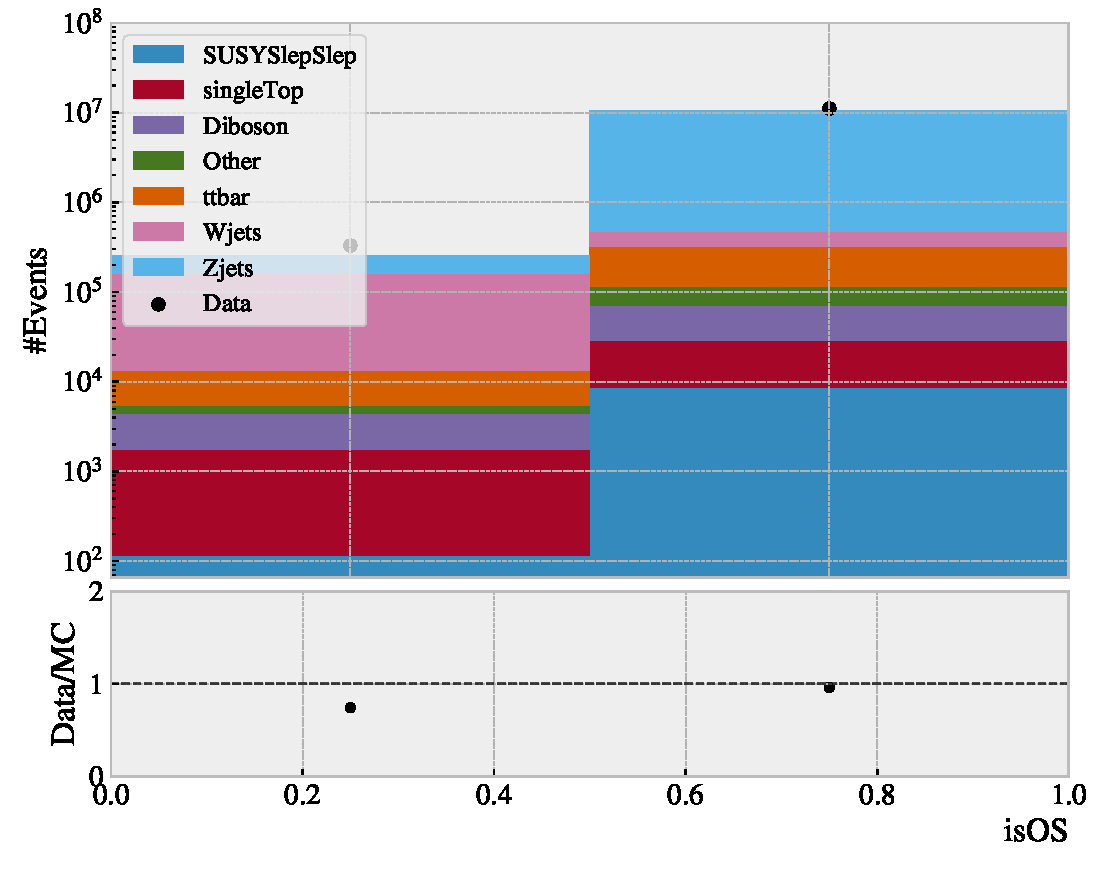
\includegraphics[width=\textwidth]{Figures/Cuts/isOS.pdf} 
         \caption{}
         \label{fig:Cuts_isOS}
     \end{subfigure}
    }
    \caption{The distribution of nr of B-jets \ref{fig:Cuts_bTag}, jets with a transverse momentum above 20[GeV] \ref{fig:Cuts_jet20}  and 60[GeV] \ref{fig:Cuts_jet60} and the number of lepton pairs with opposite or equal charge \ref{fig:Cuts_isOS} for the MC and real data. Additionally the ratio of data over MC is plotted under each distribution histogram.}
    \label{fig:var2}
\end{figure}
In figure \ref{fig:var2} we plot the distribution of the nr of B-jets \ref{fig:Cuts_bTag}, the number of jets with transverse momentum larger than 20GeV \ref{fig:Cuts_jet20}
and 60GeV \ref{fig:Cuts_jet60} and the number of events with same or opposite sign \ref{fig:Cuts_isOS}. From all the plots in figure \ref{fig:var2}, we observe the same as for figure \ref{fig:var1}. In other words we observe a clear similarity between the MC and real data. From our study of the distribution of different variables we can conclude that the MC adequately resembles the real data.
\subsection{Cuts for AR}
In this section I will present the cuts made to define the AR as well as the result from applying them to the full data set. By studying the distribution plots in figure \ref{fig:var1} and \ref{fig:var1}, I aimed to remove as much of the background by making cuts before any of the peaks for the SUSY signal. By doing so I defined the region as presented by the cuts in table \ref{table:AR}. Note that the cut applied on the missing transverse energy is the only case were a upper-limit is defined. This was done as an attempt to remove regions were the MC and real data differ in a unsystematic way.
\bgroup
\title{TBD}
{\tabcolsep=20pt
\begin{table}
    \caption{Feature cuts in AR}
    \label{table:AR}
    \centering 
    \begin{threeparttable}
    \begin{tabular}{ccc}
    Features & & Thresholds\\
     \midrule\midrule
    $\bar{E}_t$   & &  $> 50, \ < 250[GeV]$  \\%new row
    \cmidrule(l  r ){1-3}
     $P_t \ (1)$ & &  $> 80[GeV]$  \\ 
    \cmidrule(l r ){1-3}
     $P_t \ (2)$ & & $>25[GeV]$  \\ 
    \cmidrule(l r ){1-3}
    $m_{ll}$ & & $>120[GeV]$  \\
    \cmidrule(l r ){1-3}
    $m_{T2}$  & & $>150[GeV]$ \\
    \cmidrule(l r ){1-3}
    $Nr\ B-Jet$ & & $<2$  \\ 
    \cmidrule(l r ){1-3}
    $isOS$ & & $True$  \\ 
    \cmidrule(l r ){1-3}
    $isSS$ & & $False$  \\ 
    \midrule\midrule
    \end{tabular}
    \end{threeparttable}
\end{table}
}
\egroup
\newline
By applying the cuts for the AR a great amount of the data was removed. The resulting reduction on each channel is presented in table \ref{table:AR_result}. From the table we can see that Z+jets and W+jets was effected the most, removing more than $99.99\%$ from both channels. Dibson and ttbar were reduced $96\%$ and $94\%$ respectively. As expected this channels are harder to remove given their similiarity to the signal. The others channels was like the Z/W+jets channel almost completely removed. The SUSY-signal was however only reduced by $74\%$ making it the second largest channel in the AR, only beaten by the W+jets channel.
\bgroup
\title{TBD}
{\tabcolsep=20pt
\begin{table}
    \caption{Events analysis of MC-data in total and in AR}
    \label{table:AR_result}
    \begin{threeparttable}
    \makebox[\linewidth][c]{%
    \begin{tabular}{c c c c}
    \textbf{Channel} & \textbf{Nr Event total} & \textbf{Nr Events AR} & \textbf{Reduction [\%]}\\
     \midrule\midrule
    $Diboson$   & $4.5\times 10^{4}$ & $1.5\times 10^{3}$ &  $96\%$  \\%new row
    \cmidrule(l  r ){1-4}
     $ttbar$ & $2.1\times 10^{5}$ & $1.1\times 10^{4}$ & $94\%$  \\ 
    \cmidrule(l r ){1-4}
    $Z+jets$ & $1.0\times 10^{7}$ & $1.9\times 10^{3}$ & $99\%$   \\ 
    \cmidrule(l r ){1-4}
    
    $W+jets$ & $1.0\times 10^{7}$ & $2.7\times 10^{3}$ & $99\%$  \\ 
    \cmidrule(l r ){1-4}
    
    $Others$  & $3.7\times 10^{5}$ & $6.2\times 10^{1}$ & $99\%$ \\

    \cmidrule(l r ){1-4}

    $SUSYSlepSlep$  &  $8.8\times 10^{3}$ & $2.3\times 10^{3}$ & $74\%$ \\
    \midrule\midrule
    \end{tabular}
    }
    \end{threeparttable}
\end{table}
}
\egroup
\subsection{Training and validation}\label{subsec:training}
As mentioned in section \ref{sec:DH}, all training, validation and testing was done in in the AR. Firstly I preformed a fit of the classifier on the training set, containing $80\%$ of the signal and background. After training I plotted the distribution as well as the ROC-curve of the output from the classifier from the training data. The results are shown in figure \ref{fig:XGB_dist_training} and \ref{fig:XGB_dist_validation} . Figure \ref{fig:XGB_dist_training} shows a clear separation between the background and signal. This is evident from the ROC-curve which creates an area of 0.985. 
\begin{figure}
    \makebox[\linewidth][c]{%
     \centering
     \begin{subfigure}[b]{.6\textwidth}
         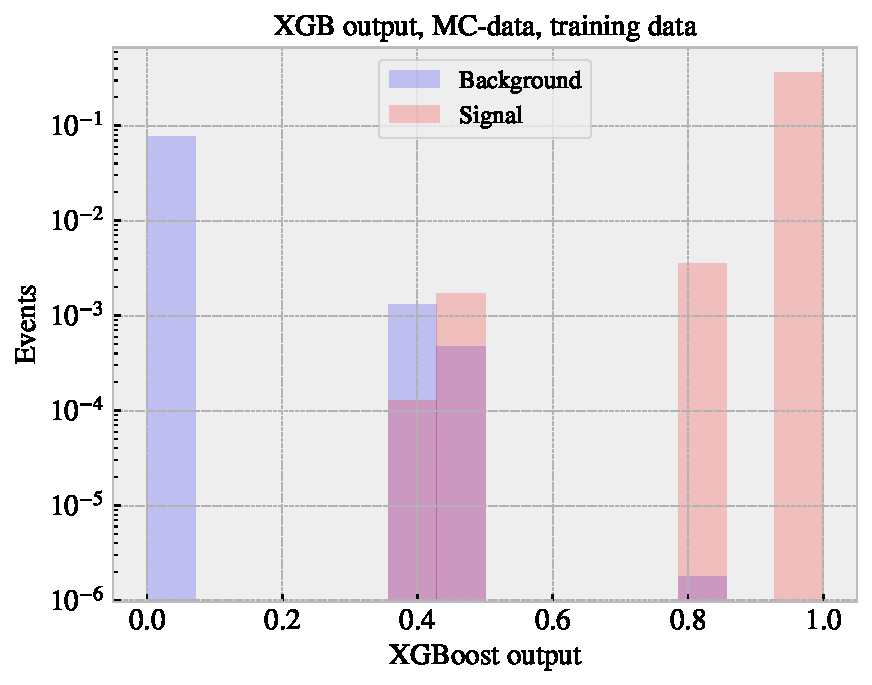
\includegraphics[width=\textwidth]{Figures/Training/train.pdf}
         \caption{}
         \label{fig:XGB_dist_training}
     \end{subfigure}
     \hfill
     \begin{subfigure}[b]{.6\textwidth}
         \includegraphics[width=\textwidth]{Figures/Training/train_ROC.pdf}
         \caption{}
         \label{fig:XGB_ROC_training}
     \end{subfigure}
    }
    \caption{The output distribution \ref{fig:XGB_dist_training} and the ROC-curve \ref{fig:XGB_ROC_training} produced by the XGBoost-classifier on training data. }
\end{figure}
\newline
After training and analysing the reuslts on the training data, I create similar plots for the validation data. The distribution and ROC-curve is displayed in figures \ref{fig:XGB_dist_validation}
and \ref{fig:XGB_ROC_validation}. In figure \ref{fig:XGB_dist_validation} we see a clear separation between the signal and background, although not as prominent as in the training data. From figure \ref{fig:XGB_ROC_validation} we see that the classifier achieves an excellent ROC-curve area of 0.963. The optimal threshold should be placed in the area where the ratio of true positive divided by false positive is highest. From figure \ref{fig:XGB_ROC_validation} we can observe that this is in the region of [0.85, 0.95].
\\
It is clear from the validation data that the XGBoost has picked up differences in trend for the signal and background and will be an can be used as a tool in the hope to create a effective signal region. 
\newline
\begin{figure}
    \makebox[\linewidth][c]{%
     \centering
     \begin{subfigure}[b]{.6\textwidth}
         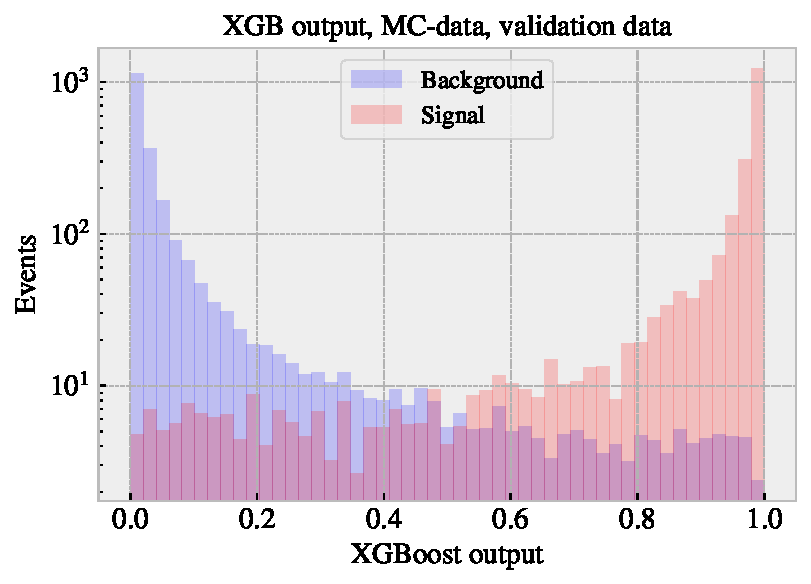
\includegraphics[width=\textwidth]{Figures/Training/validation.pdf}
         \caption{}
         \label{fig:XGB_dist_validation}
     \end{subfigure}
     \hfill
     \begin{subfigure}[b]{.6\textwidth}
         \includegraphics[width=\textwidth]{Figures/Training/validation_ROC.pdf}
         \caption{}
         \label{fig:XGB_ROC_validation}
     \end{subfigure}
    }
    \caption{The output distribution \ref{fig:XGB_dist_validation} and the ROC-curve \ref{fig:XGB_ROC_validation} produced by the XGBoost-classifier on validation data.}
\end{figure}
Finally we plot the distribution of all the background data in figure \ref{fig:XGB_dist_background}. The figure displays the classifiers ability to separate more than $90\%$ of the MC background to the lowest values of the output. 
\begin{figure}
    \centering
    \includegraphics[width=0.8\linewidth]{Figures/Training/BackgroundMC.pdf}
    \caption{The output distribution of the XGBoost on all background MC data.}
    \label{fig:XGB_dist_background}
\end{figure}
\subsection{Cuts for SR1}
After training our XGBoost-classifier on the MC we can apply it on the real data and compare. In figure \ref{fig:XGB_SR1} I have plotted the distribution of the XGBoost output for both the MC background and the real data. Under the figure we see the ratio-plot between the two in each bin. From the distribution and ratio plot we see a clear similarity between the output for the MC and real data. Given the goal of comparing the two in different region, it is vital that the XGboost treats both similarly.
\\
In the distribution plot in figure \ref{fig:XGB_SR1} we also observe that most of the data is centered around the lower values of the output. Comparing to the distribution plot of the MC-signal in figure \ref{fig:XGB_SUSY}, we can see that the XGBoost classier has accurately separated most of the background from the signal. Note also that the MC-background in these plots are from the AR, meaning the background data in the plots are the events most similar to the signal, making the results of the XGBoost that much more impressive. 
\\
Finally in figure \ref{fig:XGB_SR1}, I plotted a dotted line representing the cut of the ML-output, defining the SR1. After some testing I found that the optimal threshold was for output values around 0.875, which inline with our observations made from the ROC-curve in section \ref{subsec:training}. This means that SR1 is defined as the data satisfying the AR requirements (see table \ref{table:AR}), as well as having a XGBoost output above 0.875. Using these requirements for SR1, we get the results as displayed in table \ref{table:SR1_R}.
\\
\begin{figure}
    \makebox[\linewidth][c]{%
     \centering
     \begin{subfigure}[b]{.6\textwidth}
         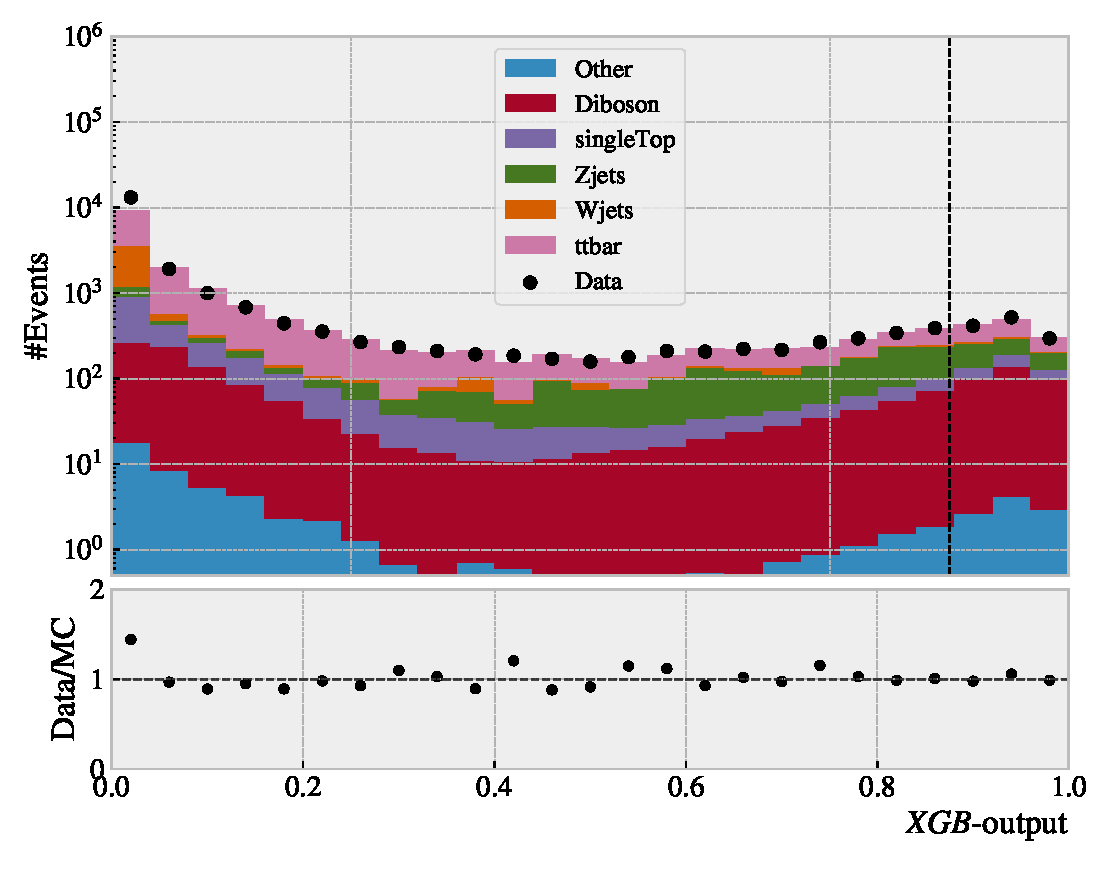
\includegraphics[width=\textwidth]{Figures/Results/XGB_dist.pdf}
         \caption{}
         \label{fig:XGB_SR1}
     \end{subfigure}
     \centering
     \begin{subfigure}[b]{.65\textwidth}
         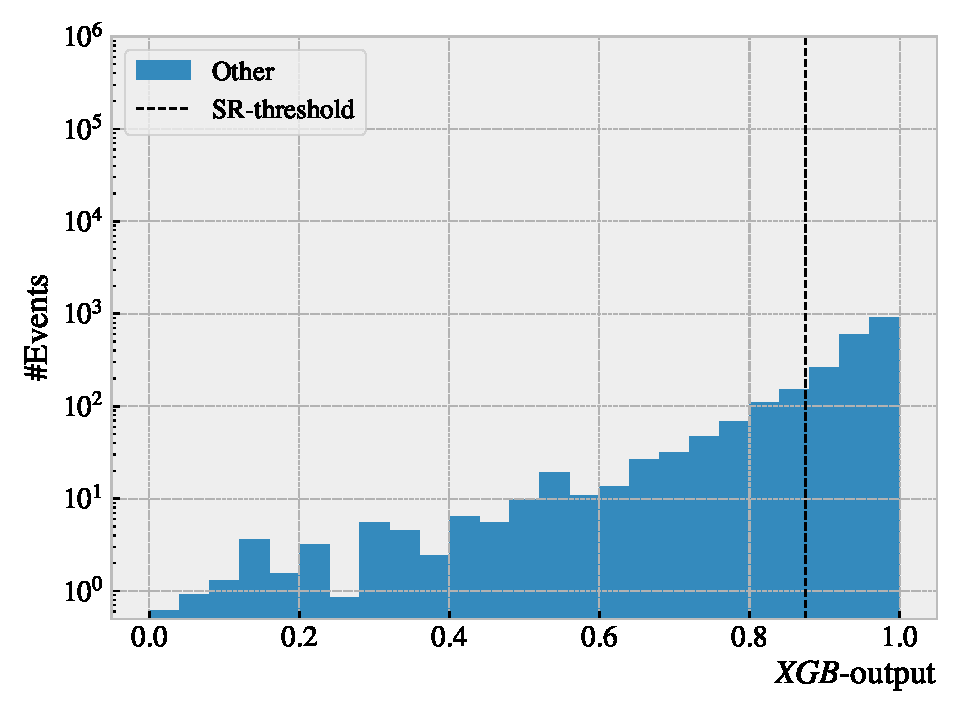
\includegraphics[width=\textwidth]{Figures/Results/XGB_SUSY.pdf}
         \caption{}
         \label{fig:XGB_SUSY}
     \end{subfigure}
    }
    \caption{XGBoost output distribution for MC and data \ref{fig:XGB_SR1} and the SUSYSlepSlep-MC \ref{fig:XGB_SUSY} in SR1.}
\end{figure}
\begin{figure}
\bgroup
In table \ref{table:SR1_R}, we observe that all background MC was reduced down to bellow 500 events, whereas the MC-signal still contains almost 2000 events. By comparison to the cuts made for the AR, the XGboost-classifer was able to cut far more efficiently, again keeping in mind that the data it was given is the background most similar to the signal. Although SR1 only cut $21\%$ of the signal, it still cut mor than $75\%$ of all the background, even reducing channels like ttbar and W+jets by $96\%$ and $99\%$.
\\
As was briefly mentioned in section \ref{subsec:WZjets}, the W/Z+jets-channels are normally negligible in searches such as these.  In articles like the ones from ATLAS in 2020 \cite{Aad_2020} or the work by Eirik Gramstad in 2013 \cite{Gramstad:2013loc}, cuts are normally made on different variables for the jets to reduce W/Z+jets-channels, or even ttbar. This would make the diboson-channel the largest irreducible background. In the data set used for this analysis, there was not enough features for the jets to reduce W/Z+jets- or ttbar-channels to a similar degree. Therefore ttbar and Z+jets effect the signal region more than usual. On the other hand the classifier was able to reduce the W+jets-channel to an almost negligible amount, 40. 
\title{TBD}
{\tabcolsep=20pt
\begin{table}
    \caption{Events analsysis of MC-data in total and in SR1}
    \centering 
    \begin{threeparttable}
    \makebox[\linewidth][c]{%
    \begin{tabular}{c c c c}
    \textbf{Channel} & \textbf{Nr Event AR} & \textbf{Nr Events SR1} & \textbf{Reduction [\%]}\\
     \midrule\midrule
    $Diboson$   & $1.5\times 10^{3}$ & $3.3\times 10^{2}$ &  $78\%$  \\%new row
    \cmidrule(l  r ){1-4}
     $ttbar$ & $1.1\times 10^{4}$ & $4.4\times 10^{2}$ & $96\%$  \\ 
    \cmidrule(l r ){1-4}
    $Z+jets$ & $1.9\times 10^{3}$ & $3.1\times 10^{2}$ & $83\%$   \\ 
    \cmidrule(l r ){1-4}
    
    $W+jets$ & $2.7\times 10^{3}$ & $4.0\times 10^{1}$ & $99\%$  \\ 
    \cmidrule(l r ){1-4}

    $Others$  & $6.2\times 10^{1}$ & $1.0\times 10^{1}$ & $84\%$ \\
    \cmidrule(l r ){1-4}

    $SUSYSlepSlep$  &  $2.3\times 10^{3}$ & $1.8\times 10^{3}$ & $21\%$ \\
    \midrule\midrule
    \end{tabular}
    }
    \end{threeparttable}
    \label{table:SR1_R}
\end{table}
}
\egroup
\end{figure}
\subsection{Cuts for SR2}
Producing any result using the rectangle cut only approach, required a much stricter strategy than was the case for AR. The cuts made in this section were characterized by the attempt to reduce the amount of background in AR and thereby subsequently reducing any relative difference between the MC and real data. The resulting cuts for SR1 are displayed in table \ref{table:AR}, which are made in addition to the AR cuts. \\
\bgroup
\title{TBD}
{\tabcolsep=20pt
\begin{table}
    \caption{Feature cuts in SR2}
    \label{table:AR}
    \centering 
    \begin{threeparttable}
    \begin{tabular}{ccc}
    \textbf{Features} & & \textbf{Thresholds}\\
     \midrule\midrule
    $\bar{E}_t$   & &  $ > 75, \ < 150[GeV]$  \\%new row
    \cmidrule(l  r ){1-3}
     $P_t \ (1)$ & &  $< 200[GeV]$  \\ 
    \cmidrule(l r ){1-3}
     $P_t \ (2)$ & & $> 60[GeV]$  \\ 
    \cmidrule(l r ){1-3}
    $m_{ll}$ & & $< 300[GeV]$  \\
    \cmidrule(l r ){1-3}
    $Nr\ B-Jet\  (P_t>20GeV$) & & $< 2$  \\ 
    \midrule\midrule
    \end{tabular}
    \end{threeparttable}
\end{table}
}
\egroup
As discussed in the analysis of feature distribution \ref{subsec:MCandData}, there seemed to be the most unsystematic deviation between MC and data in the areas with highest energies. This explains that most of the cuts added to the region are upper limits. Although this upper-limits reduce the possibility of fluctuation differences in the data, one also risk removing a large amount of the higher mass sleptons and neutralinos. 
\\
The results from defining the new region SR2 are presented in table \ref{table:SR2_R}. The table shows a larger reduction on all channels but the W+jets, compared to the SR1 region. All channels are reduced by more than $90\%$. The cost of the reduction of the background, is the reduction of the signal which is now more than $80\%$.
\bgroup
\title{TBD}
{\tabcolsep=20pt
\begin{table}
    \caption{Events analsysis of MC-data in total and in SR2}
    \label{table:SR2_R}
    \centering 
    \begin{threeparttable}
    \makebox[\linewidth][c]{%
    \begin{tabular}{c c c c}
    \textbf{Channel} & \textbf{Nr Event AR} & \textbf{Nr Events SR2} & \textbf{Reduction [\%]}\\
     \midrule\midrule
    $Diboson$   & $1.5\times 10^{3}$ & $1.4\times 10^{2}$ &  $90\%$  \\%new row
    \cmidrule(l  r ){1-4}
     $ttbar$ & $1.1\times 10^{4}$ & $5.8\times 10^{2}$ & $94\%$  \\ 
    \cmidrule(l r ){1-4}
    $Z+jets$ & $1.9\times 10^{3}$ & $1.0\times 10^{2}$ & $94\%$   \\ 
    \cmidrule(l r ){1-4}
    
    $W+jets$ & $2.7\times 10^{3}$ & $1.2\times 10^{2}$ & $95\%$  \\ 
    \cmidrule(l r ){1-4}

    $Others$  & $6.2\times 10^{1}$ & $5.0\times 10^{0}$ & $92\%$ \\
    \cmidrule(l r ){1-4}

    $SUSYSlepSlep$  &  $2.3\times 10^{3}$ & $4.2\times 10^{2}$ & $81\%$ \\
    \midrule\midrule
    \end{tabular}
    }
    \end{threeparttable}
\end{table}
}
\egroup
\subsection{Discovery or exclusion}
In table \ref{table:SR1_SR2} I have written the resulting MC-background and data in both SR1 and SR2, along with the resulting significance. The Significance was calculated using equation \ref{eq:Z}. From the table we see that both SR1 and SR2 cut a relatively similar amount of events for both MC and data. SR1 achieved a significance of 0.25 whereas SR2 achieved a significance of 1.20, which are both far from 5. Neither of the regions found a deviation between the MC and data worth any further search as far as discovery is concerned.
\\
\bgroup
\title{TBD}
{\tabcolsep=20pt
\begin{table}
    \caption{Final result of MC and data in SR1 an SR2}
    \label{table:SR1_SR2}
    \centering 
    \begin{threeparttable}
    \begin{tabular}{cccc}
    \textbf{Region} & \textbf{MC} & \textbf{Data} & \textbf{Significance (Z)}\\
    \midrule\midrule
    $SR1$   & $1266$ &  $1284$ & 0.25 \\%new row
    \cmidrule(l  r ){1-4}
    $SR2$ & $1097$ &  1174 & 1.20 \\ 
    \midrule\midrule
    \end{tabular}
    \end{threeparttable}
\end{table}
}
\egroup
Given the lack of discovery I aim to exclude certain masses for the SUSY model. I do this by studying each pair of different masses for the slepton and the neutralino, discussed in \ref{sec:SUSY}. Before I can calculate the limits and check for exclusion, I need to calculate the efficiency of each pair. 
\\
In table \ref{table:eff} I displayed the number of signal events in each region for each mass pair, along with the resulting efficiency. Already we see that SR1 has cut far less signal than SR2. In addition we observe that most of events left are in the smaller mass range. 
\bgroup
\centering
\title{TBD}
{\tabcolsep=20pt
\begin{table}
    \centering
    \caption{Exclusion of slepton and neutralino massses.}
    \centering 
    \begin{threeparttable}
    \makebox[\linewidth][c]{%
    \begin{tabular}{ccc}
    \textbf{Masses[GeV]} &  \textbf{Events in SR1 [efficiency]} & \textbf{Events in SR2 [efficiency]}  \\
     \midrule\midrule
    $m_{\tilde{l}} = 100$, $m_{\tilde{\chi}} = 50$   & 461 [0.173]  & 105 [0.028]   \\%new row
    \cmidrule(l  r ){1-3}
     $m_{\tilde{l}} = 100.5$, $m_{\tilde{\chi}}  = 1$ & 913 [0.280] &  239 [0.057]  \\ 
    \cmidrule(l r ){1-3}
    $m_{\tilde{l}} = 200$, $m_{\tilde{\chi}}  = 100$ & 144 [0.461] & 37 [0.100]  \\ 
    \cmidrule(l r ){1-3}

    $m_{\tilde{l}} = 200.5$, $m_{\tilde{\chi}} = 1$  & 203 [0.571] & 30 [0.075]   \\% end of rows
    \cmidrule(l r ){1-3}
    
    $m_{\tilde{l}} = 300$, $m_{\tilde{\chi}}  = 200$  & 30 [0.484] &   7 [0.102] \\
    \cmidrule(l r ){1-3}
    
    $m_{\tilde{l}} = 300.5$, $m_{\tilde{\chi}}  = 1$  & 37 [0.529]  &   2 [0.032] \\
    \cmidrule(l r ){1-3}
    
    $m_{\tilde{l}} = 400$, $m_{\tilde{\chi}}  = 300$  & 8 [0.484]  &   2 [0.093] \\
    \cmidrule(l r ){1-3}
    
    $m_{\tilde{l}} = 500$, $m_{\tilde{\chi}}  = 100$  & 3 [0.523] &   0 [0.000] \\
    \cmidrule(l r ){1-3}
    
    $m_{\tilde{l}} = 500$, $m_{\tilde{\chi}}  = 100$  &  2 [0.475] &   0 [0.000] \\
    \cmidrule(l r ){1-3}
    
    $m_{\tilde{l}} = 500.5$, $m_{\tilde{\chi}}  = 1$  & 2 [0.491]  &   0 [0.000] \\
    \cmidrule(l r ){1-3}
    
    $m_{\tilde{l}} = 600$, $m_{\tilde{\chi}}  = 1$  &  1 [0.322]  &   0 [0.000] \\
    \cmidrule(l r ){1-3}
    
    $m_{\tilde{l}} = 600$, $m_{\tilde{\chi}}  = 300$  & 1 [0.309] &   0 [0.000] \\
    \cmidrule(l r ){1-3}
    
    $m_{\tilde{l}} =  700$, $m_{\tilde{\chi}}  = 300$  & 0 [0.00]  &   0 [0.000] \\
    \cmidrule(l r ){1-3}
    
    $m_{\tilde{l}} =  700.5$, $m_{\tilde{\chi}}  = 1$  &  0 [0.00]
    &   0 [0.000] \\
    \midrule\midrule
    \end{tabular}
    }
    \end{threeparttable}
    \label{table:eff}
\end{table}
}
\egroup
Using the number of events and efficiency I calculated the limits for each off the mass pair. To visualize the reult I created two plots for each of the regions. The plots visualize the limits for each pair both for a $95\%$ and $87\%$ confidence. Any mass pair with a cross section above any of the aforementioned lines, is excluded up to that confidence. 
\\
In figure \ref{fig:ExlusionSR1} I plotted the result for SR1. From the figure we observe that one of the mass pairs are excluded up to $95\%$ confidence, namely the pair with a slepton mass of $100.5$GeV and $1$GeV nautralino mass. The rest of the mass pairs were not excluded up to this confidence, although one was almost excluded up to $87\%$ confidence (200.5Gev and 1GeV).
\begin{figure}
    \makebox[\linewidth][c]{%
     \centering
     \begin{subfigure}[b]{\textwidth}
         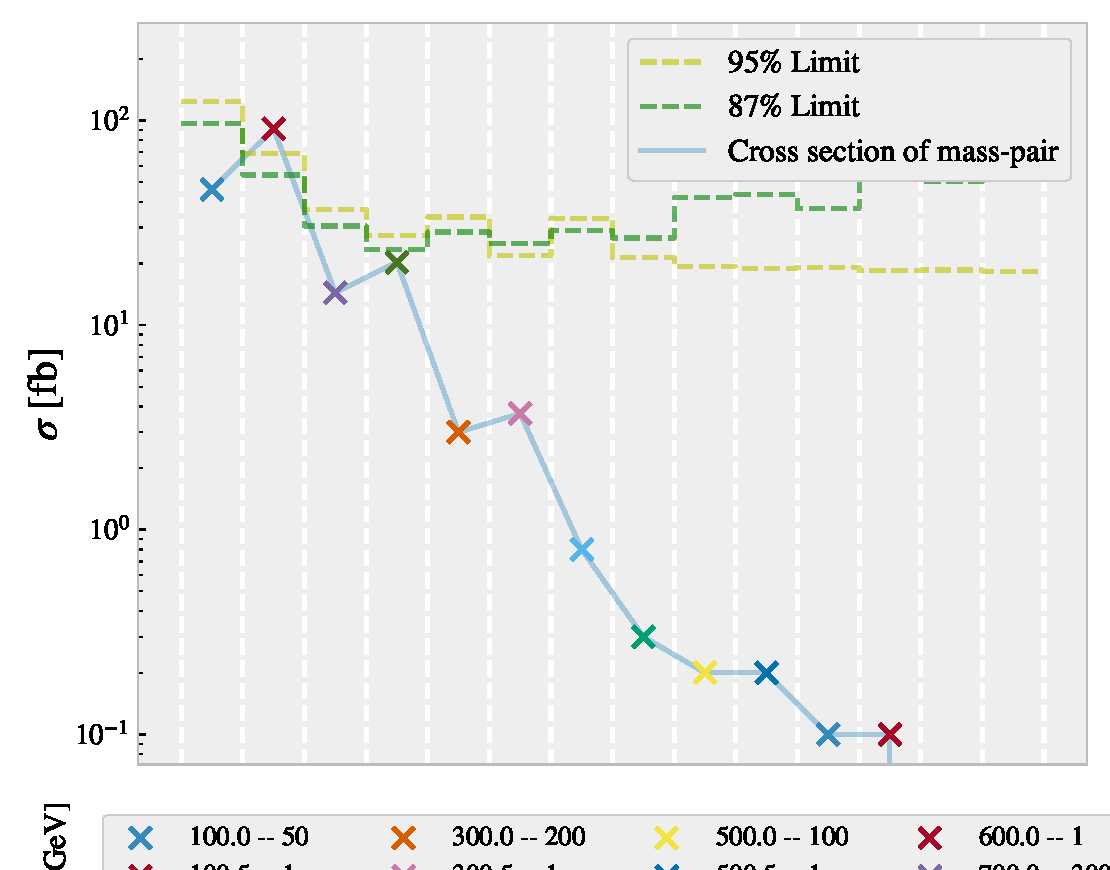
\includegraphics[width=\textwidth]{Figures/Results/ExlusionEvents.pdf}
     \end{subfigure}
     }
     \caption{Visualization of crossection of each mass-pair in SR2 with each corresponding exclusion limit up to $95\%$ and $87\%$.}
     \label{fig:ExlusionSR1}
\end{figure}
\begin{figure}
    \makebox[\linewidth][c]{%
     \centering
     \begin{subfigure}[b]{\textwidth}
         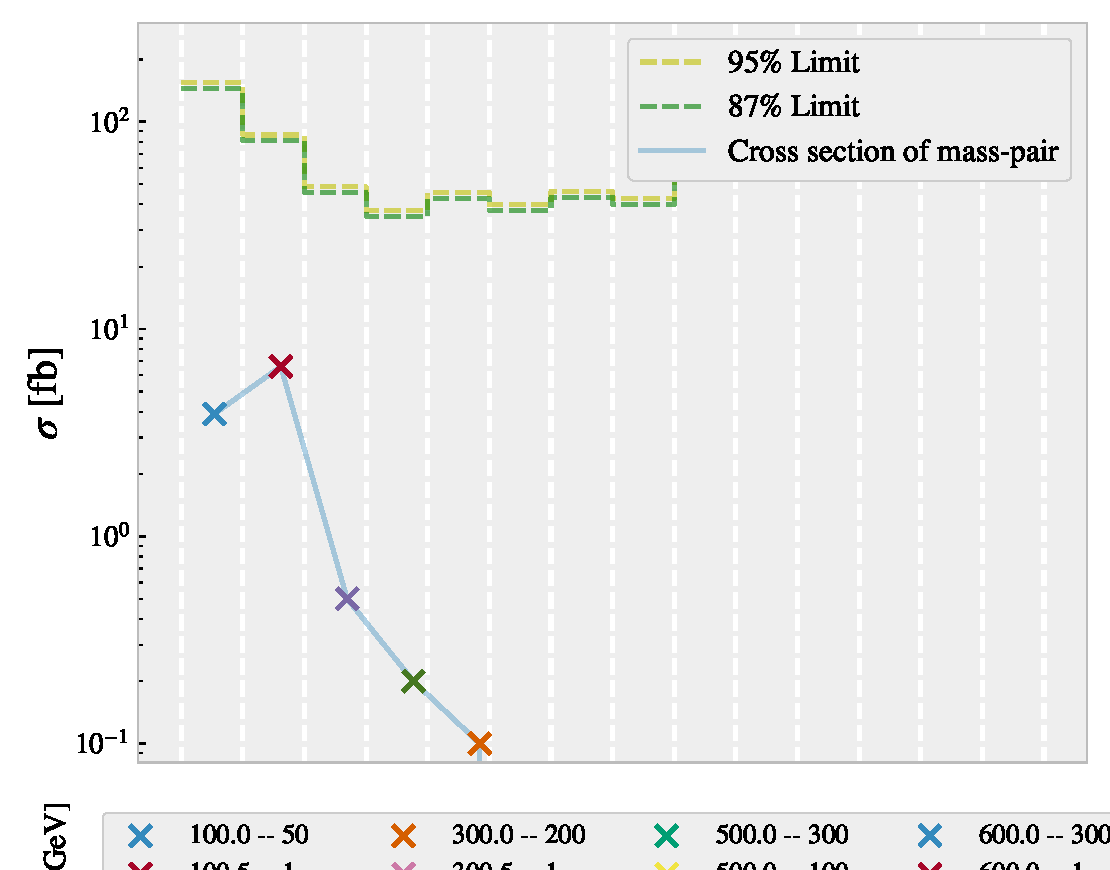
\includegraphics[width=\textwidth]{Figures/StatAnal/ExlusionEvents_nML.pdf}
         \caption{Visualization of crossection of each mass-pair in SR3 with each corresponding exclusion limit up to $95\%$ and $87\%$.}
         \label{fig:ExlusionSR2}
     \end{subfigure}
    }
\end{figure}


\subsection{The way forward}
\begin{itemize}
    \item More data
    \item Individual SR for each mass. Some masses prefer a stricter threshold on ML
    \item New way of handling negative weights. Cell resampling (https://arxiv.org/pdf/2109.07851.pdf)
    \item More data on Jets, possibly exclude more Z+Jets and W+Jets before ML-Cut
    \item accurate uncertainty 
\end{itemize}

\section{Conclusion}
\newpage
\printbibliography

\end{document}
